\section{Molecular crystals}\label{sec:16.4}

Anthracene, C$_{14}$H$_{10}$, is three benzene rings fused in a row. Its molecules stack in a monoclinic crystal, two to a cell, and the crystal keeps much of the molecule's spectrum: the lowest singlet absorption lies at \SI{3.1}{eV} in the crystal against \SI{3.5}{eV} in the gas~\cite[Tables~I and~III]{rangel2016structural}. A particle must carry $2\times\SI{3.1}{eV}/v_{\mathrm{max}}^2 = \SI{0.883}{MeV}$ to make this excitation (\cref{eq:1.3-mmin}), and an organic crystal turns a large fraction of its singlet excitations into scintillation photons that a photodetector can count, at least 63 percent of them in trans-stilbene~\cite[Sect.~IV\,B]{blanco2021dark}. The electrons that dark matter excites near threshold are in $\pi$ orbitals perpendicular to the flat molecule, and all molecules of the crystal point along two directions, so the rate depends on the angle at which the dark-matter wind meets the molecular planes, and this angle turns with the Earth. The excited electron stays on its molecule, bound to the hole it left: an excitation that stays on one molecule is a \emph{Frenkel exciton}. (The vacancy--interstitial pair of \cref{sec:7.4} is an unrelated object of the same name.)

\subsection{Molecular-basis Bethe--Salpeter equation}\label{sec:16.4-bse}

\Cref{eq:4.9-bse} holds in any basis of electron--hole pairs, and for a molecular crystal the natural one is localized. Combine the occupied Bloch states into orbitals $\phi_{v\mathfrak{o}}$ centered on molecule $\mathfrak{o}$, and the empty ones into orbitals $\phi_{c\mathfrak{o}}$, where $\mathfrak{o} = 1,\dots,N_{\mathrm{mol}}$ labels the molecules of the cell at positions $\vect{r}_{\mathfrak{o}}$ and the cell index is kept implicit. A pair is then an electron in $\phi_{c\mathfrak{o}'}$ and a hole in $\phi_{v\mathfrak{o}}$. If $\mathfrak{o}' = \mathfrak{o}$ the electron stays on the molecule where the hole is; if $\mathfrak{o}' \ne \mathfrak{o}$ the pair is a \emph{charge-transfer} pair, with the electron on a neighbor at a distance $d$.

The kernels of \cref{eq:4.9-kernels} now take a simple form when the orbitals of different molecules do not overlap. The direct kernel contains the overlap densities $\phi_{c\mathfrak{o}'}^*\phi_{c\mathfrak{o}'''}$ and $\phi_{v\mathfrak{o}}^*\phi_{v\mathfrak{o}''}$, which vanish unless the electron and the hole each stay on their molecule. It therefore acts within one molecule, as the intramolecular attraction, and between the partners of a charge-transfer pair, as their screened attraction at distance $d$. The exchange kernel contains the transition densities $\phi_{c\mathfrak{o}'}^*\phi_{v\mathfrak{o}}$, which vanish for a charge-transfer pair; on one molecule they are the charge distribution of a molecular transition, and exchange couples these molecular transitions on different molecules through their Coulomb interaction. In the limit of zero overlap the charge-transfer pairs decouple, and the problem separates into two steps.

The first step is the molecule. Its own block of $H^{\mathrm{exc}}$, with both kernels, gives the singlet excited states $\mathfrak{x}$ of one molecule in the crystal, with energies $E_{\mathfrak{x}}$ and transition densities $\rho^{(\mathfrak{o})}_{0\mathfrak{x}}(\vect{r}) = \langle\mathfrak{x}|\hat{\nd}_e(\vect{r})|0\rangle$. The Fourier transforms of the transition densities are the molecular form factors,
\begin{equation}
  f^{(\mathfrak{o})}_{0\mathfrak{x}}(\vect{q}) = \int\dd^3r\;\ee^{\ii\vect{q}\cdot(\vect{r} - \vect{r}_{\mathfrak{o}})}\,\rho^{(\mathfrak{o})}_{0\mathfrak{x}}(\vect{r}) = \Bigl\langle\mathfrak{x}\Bigl|\sum_j\ee^{\ii\vect{q}\cdot(\vect{r}_j - \vect{r}_{\mathfrak{o}})}\Bigr|0\Bigr\rangle ,
  \label{eq:16.4-ff}
\end{equation}
with the sum over the electrons of the molecule. The singlet factor $\sqrt{g_{\mathrm{deg}}}$ of \cref{sec:10.5} is inside $f$, since $\langle\mathfrak{x}|$ is the full many-electron state. Molecules related by a rotation $\mathsf{R}_{\mathfrak{o}}$ have form factors related by $f^{(\mathfrak{o})}_{0\mathfrak{x}}(\vect{q}) = f_{0\mathfrak{x}}(\mathsf{R}_{\mathfrak{o}}^{-1}\vect{q})$, and at small $q$ each starts as $\ii\vect{q}\cdot\vect{d}_{\mathfrak{x}}$, with $\vect{d}_{\mathfrak{x}} = \langle\mathfrak{x}|\sum_j(\vect{r}_j - \vect{r}_{\mathfrak{o}})|0\rangle$ the transition dipole that fixes the oscillator strength \cref{eq:4.3-osc}.

The second step is the crystal. A molecular excitation on $\mathfrak{o}$ can move to $\mathfrak{o}'$ when its transition density and that of the receiving molecule interact, and the Bloch combinations of crystal momentum $\vect{Q}$ diagonalize the translations. The Frenkel Hamiltonian is
\begin{equation}
  \begin{gathered}
  H^{\mathrm{F}}_{\mathfrak{o}\mathfrak{x},\mathfrak{o}'\mathfrak{x}'}(\vect{Q}) = E_{\mathfrak{x}}\,\delta_{\mathfrak{o}\mathfrak{o}'}\delta_{\mathfrak{x}\mathfrak{x}'} + \mathfrak{J}_{\mathfrak{o}\mathfrak{x},\mathfrak{o}'\mathfrak{x}'}(\vect{Q}) ,\\
  \mathfrak{J}_{\mathfrak{o}\mathfrak{x},\mathfrak{o}'\mathfrak{x}'}(\vect{Q}) = {\sum_{\vect{R}}}'\,\ee^{\ii\vect{Q}\cdot\vect{R}}\int\dd^3r\,\dd^3r'\;\rho^{(\mathfrak{o})}_{0\mathfrak{x}}(\vect{r})^*\,\frac{e^2}{4\pi|\vect{r} - \vect{r}' - \vect{R}|}\,\rho^{(\mathfrak{o}')}_{0\mathfrak{x}'}(\vect{r}') ,
  \end{gathered}
  \label{eq:16.4-HF}
\end{equation}
where the prime drops the term $\vect{R} = 0$, $\mathfrak{o}' = \mathfrak{o}$, since a molecule's interaction with itself is already in $E_{\mathfrak{x}}$. The coupling $\mathfrak{J}$ is the exchange kernel $g_{\mathrm{deg}}K^{\mathrm{x}}$ of \cref{eq:4.9-kernels} between molecules, written in real space; as there, its long-wavelength part, the Fourier component at $\vect{Q}$ itself, is removed and kept in $\varepsilon_{\mathrm{mac}}$. The lattice sum converges only conditionally, and in practice it is done by Ewald's method. The eigenvectors $A^\lambda_{\mathfrak{o}\mathfrak{x}}(\vect{Q})$ and energies $E_\lambda(\vect{Q})$ of $H^{\mathrm{F}}$ are the Frenkel excitons. A molecular level becomes $N_{\mathrm{mol}}$ exciton bands. At $\vect{Q} \to 0$ the exciton bands give the \emph{Davydov splitting} of the absorption line of the molecular level into components, and in a cell with two inequivalent orientations the components absorb light of different polarizations.

The molecular energies and transition densities are the material input. They come from the $GW$ and Bethe--Salpeter equations solved for one molecule in a basis of atom-centered Gaussian orbitals, with singlet energies typically within \SIrange{0.1}{0.3}{eV} of measurement. The crystal enters either as the reaction field of a polarizable medium or through a calculation of the whole periodic crystal (\cref{app:E.6}). In anthracene the environment lowers the fundamental gap, the difference between ionization energy and electron affinity, from \SI{6.9}{eV} in the gas to 3.9--\SI{4.2}{eV} in the crystal~\cite[Tables~I--III]{rangel2016structural}, since the polarization of the neighbors stabilizes a separated electron and hole far more than a neutral excitation. A periodic $GW$ calculation followed by the Bethe--Salpeter equation places the crystal's lowest singlet at \SI{3.3}{eV}, against the measured \SI{3.1}{eV}~\cite[Table~III]{rangel2016structural}.

\subsection{Frenkel-exciton rate}\label{sec:16.4-rate}

The structure factor follows from \cref{eq:4.9-S} with the molecular basis in place of the band pairs. The vertex of the pair $(\mathfrak{o},\mathfrak{x})$ at momentum transfer $\vect{q}$ is $F_{\mathfrak{o}\mathfrak{x}}(\vect{q}) = \ee^{\ii\vect{q}\cdot\vect{r}_{\mathfrak{o}}}f^{(\mathfrak{o})}_{0\mathfrak{x}}(\vect{q})$, where the phase places the molecule in the cell, and the exciton that a momentum transfer $\vect{q}$ creates has crystal momentum $\vect{q}$. Per cell of volume $\Omega$,
\begin{equation}
  S^{\mathrm{F}}(\vect{q},\omega) = \frac{2\pi}{\Omega}\sum_\lambda\frac{\bigl|\sum_{\mathfrak{o}\mathfrak{x}}A^\lambda_{\mathfrak{o}\mathfrak{x}}(\vect{q})^*\,F_{\mathfrak{o}\mathfrak{x}}(\vect{q})\bigr|^2}{|\varepsilon_{\mathrm{mac}}(\vect{q},\omega)|^2}\,\delta\bigl(\omega - E_\lambda(\vect{q})\bigr) .
  \label{eq:16.4-S}
\end{equation}
Each exciton is a coherent superposition of excitations on all molecules, and its weight carries the interference between the molecular excitations through the phases $\ee^{\ii\vect{q}\cdot\vect{r}_{\mathfrak{o}}}$. A detector does not resolve the individual excitons, however. Integrate \cref{eq:16.4-S} over an energy window $\mathcal{B}$ that contains every exciton built from a set of molecular levels and no other, and assume that $\mathfrak{J}$ couples no level of the set to a level outside it and that $\varepsilon_{\mathrm{mac}}$ does not change across the window. Since $H^{\mathrm{F}}$ is Hermitian, as in the Tamm--Dancoff form of \cref{sec:4.9}, the eigenvectors restricted to the set are then complete, $\sum_{\lambda\in\mathcal{B}}A^\lambda(A^\lambda)^\dagger = 1$, and
\begin{equation}
  \int_{\mathcal{B}}\dd\omega\;S^{\mathrm{F}}(\vect{q},\omega) = \frac{2\pi}{\Omega\,|\varepsilon_{\mathrm{mac}}(\vect{q})|^2}\sum_{\mathfrak{o}}\sum_{\mathfrak{x}\in\mathcal{B}}\bigl|f^{(\mathfrak{o})}_{0\mathfrak{x}}(\vect{q})\bigr|^2 .
  \label{eq:16.4-binned}
\end{equation}
The phases have dropped out. Once the structure factor is summed over all Davydov components and over the whole exciton band, the crystal responds as a set of independent molecules, whatever $\mathfrak{J}$ is. At $q \to 0$, where $|f_{0\mathfrak{x}}|^2 \to |\vect{q}\cdot\vect{d}_{\mathfrak{x}}|^2$, \cref{eq:16.4-binned} becomes the oscillator-strength sum rule of molecular-exciton theory: the Davydov components share the dipole strength of the $N_{\mathrm{mol}}$ molecular transitions, $\sum_{\lambda}|\hat{\vect{e}}\cdot\vect{d}_\lambda|^2 = \sum_{\mathfrak{o}}|\hat{\vect{e}}\cdot\vect{d}^{(\mathfrak{o})}_{\mathfrak{x}}|^2$ for every polarization $\hat{\vect{e}}$. The oscillator strengths themselves add up only to order $\mathfrak{J}/E_{\mathfrak{x}}$, since \cref{eq:4.3-osc} weights each component with its own energy. \Cref{eq:16.4-binned} is the same sum rule at every momentum transfer, and \cref{we:16-davydov} works it out for anthracene.

\Cref{eq:16.4-binned} needs the window to hold whole manifolds, $\varepsilon_{\mathrm{mac}}$ and $\eta$ to stay flat across it, and the vertex to be bare. Coupling to a level $\mathfrak{x}'$ outside the window mixes the amplitude $\mathfrak{J}/(E_{\mathfrak{x}} - E_{\mathfrak{x}'})$ of the level $\mathfrak{x}'$ into a state of the window, and the weight of that state changes by
\begin{equation}
  \delta W = \frac{2\Real\bigl[F_{\mathfrak{o}\mathfrak{x}}(\vect{q})^*\,\mathfrak{J}_{\mathfrak{o}\mathfrak{x},\mathfrak{o}'\mathfrak{x}'}(\vect{q})\,F_{\mathfrak{o}'\mathfrak{x}'}(\vect{q})\bigr]}{E_{\mathfrak{x}} - E_{\mathfrak{x}'}} ,
  \label{eq:16.4-borrow}
\end{equation}
which the level outside loses. This intensity borrowing is first order in $\mathfrak{J}/\Delta E$: the cross term of two amplitudes, one of them already small, is as large as the small amplitude itself. The second condition is that $\varepsilon_{\mathrm{mac}}$ and the halo factor $\eta(\vmin)$ stay constant across the window. For a rate the window is set by kinematics: at fixed $q$, $\eta(\vmin)$ changes when $\omega$ changes by about $qv_0$, which is \SI{1.6}{eV} at $q = \SI{2}{keV}$, and much faster near threshold, where $\vmin$ approaches $v_{\mathrm{max}}$. The binned form holds when the exciton bands are narrow on this scale. The third condition is the bare vertex. The literature uses the form factors of the isolated molecule, without $1/|\varepsilon_{\mathrm{mac}}|^2$ and without the local fields that $\mathfrak{J}$ produces at finite $\vect{q}$; both corrections vanish when the dark matter resolves distances shorter than a molecule, $qa_{\mathrm{mol}} \gg 1$, with $a_{\mathrm{mol}}$ the size of the molecule. The static limit of \cref{eq:4.9-eps2} shows why: $\varepsilon_{\mathrm{mac}}(\vect{q},0) - 1 = (2e^2/\Omega q^2)\sum_{\mathfrak{o}\mathfrak{x}}|f^{(\mathfrak{o})}_{0\mathfrak{x}}|^2/E_{\mathfrak{x}}$ is finite at $q \to 0$, where it is the polarizability of the molecules, and falls once the form factors pass their maximum near $q \sim 1/a_{\mathrm{mol}}$.

Insert \cref{eq:16.4-binned} for each molecular level into \cref{eq:8.2-spectrum}, with $\varepsilon_{\mathrm{mac}} = 1$ and the window shrunk to the line at $E_{\mathfrak{x}}$, together with $|\tilde V|^2 = \pi\sigmae\FDM^2/\mu_{\chi e}^2$ (\cref{eq:1.4-Vsq}); integrate over $\omega$; and write the velocity integral at fixed $\vect{q}$ as $\hat f_{\mathrm{gal}}(\vmin + v_{\mathrm{E}}\hat{\vect{q}}\cdot\hat{\vect{v}}_{\mathrm{E}})/q$, with the Radon transform $\hat f_{\mathrm{gal}}$ of \cref{sec:11.7}. The factors $2\pi\cdot\pi/(2\pi)^3$ combine into $1/4\pi$, and with $\rho_T\Omega = M_{\mathrm{cell}}$, the mass of a cell, the rate per unit target mass is
\begin{equation}
  \mathcal{R}(\hat{\vect{v}}_{\mathrm{E}}) = \frac{\rho_\chi\,\sigmae}{\mchi\,\mu_{\chi e}^2\,M_{\mathrm{cell}}}\sum_{\mathfrak{o}\mathfrak{x}}\int\frac{\dd^3q}{4\pi q}\,\FDM(q)^2\,\bigl|f^{(\mathfrak{o})}_{0\mathfrak{x}}(\vect{q})\bigr|^2\,\hat f_{\mathrm{gal}}\bigl(\vmin^{\mathfrak{x}}(q) + v_{\mathrm{E}}\,\hat{\vect{q}}\cdot\hat{\vect{v}}_{\mathrm{E}}\bigr) ,
  \label{eq:16.4-rate}
\end{equation}
with $\vmin^{\mathfrak{x}} = E_{\mathfrak{x}}/q + q/2\mchi$ and $\hat{\vect{v}}_{\mathrm{E}}$ the direction of the Earth's velocity in crystal axes. Averaged over $\hat{\vect{v}}_{\mathrm{E}}$, the angular integral of $\hat f_{\mathrm{gal}}$ gives $2\pi\eta(\vmin)$ (\cref{eq:11.7-ups}), and \cref{eq:16.4-rate} becomes $\rho_\chi\sigmae/(2\mchi\mu_{\chi e}^2M_{\mathrm{cell}})\sum\int q\,\dd q\,\eta\,\FDM^2\langle|f|^2\rangle$. This direction-averaged rate is the rate of Blanco et al.\ for a liquid of aromatic molecules~\cite[Eqs.~(11), (13), (16)--(19)]{blanco2020dark}, with $N_{\mathrm{mol}}/M_{\mathrm{cell}}$ molecules per unit mass and unit detection efficiency. \Cref{eq:16.4-rate} itself is the direction-resolved form they use for the four molecules of trans-stilbene~\cite[Eqs.~(8), (9)]{blanco2021dark}.

\subsection{Davydov splitting in anthracene}\label{sec:16.4-model}

To put numbers on these conditions we use a $\pi$-electron model of anthracene, of the kind the literature uses for benzene and trans-stilbene~\cite{blanco2020dark,blanco2021dark}. The carbon positions are those of the measured crystal structure, with $a = \SI{8.553}{\angstrom}$, $b = \SI{6.016}{\angstrom}$, $c = \SI{11.172}{\angstrom}$ and $\beta = \ang{124.6}$~\cite{brock1990temperature}, and the second molecule of the cell is the image of the first under the twofold screw axis along $b$. We use the crystal axes $a$, $b$ and $c'$, the last perpendicular to $a$ and $b$. The long axes of both molecules make \ang{31} with $c'$, their short in-plane axes make \ang{27} with $b$, and the two molecular planes meet at \ang{51.5}, the herringbone packing of the acenes. The $\pi$ orbitals are combinations of Slater $2p_z$ orbitals with effective charge $Z_{\mathrm{eff}} = 3.15$ on the 14 carbons~\cite[Eq.~(2)]{blanco2020dark}, with the nearest-neighbor resonance integral $-0.63/(m_ex^2)$ at the measured bond length $x$~\cite[Eq.~(A1)]{blanco2021dark}. A self-consistent field of the Pariser--Parr--Pople type refines the $\pi$ orbitals; it adds the repulsion between the $\pi$ electrons to the one-electron (H\"uckel) model. We use a one-center repulsion of \SI{11.13}{eV} and the Mataga--Nishimoto form of the two-center repulsion, a standard parametrization that we take as a model choice. The singlets come from all 49 single excitations of the 14 $\pi$ electrons.

The model places the lowest singlet at \SI{3.85}{eV}, \SI{0.35}{eV} above the measured gas value. For the binned form we shift all levels down by \SI{0.75}{eV}, so that the lowest singlet lies at the measured crystal absorption, \SI{3.1}{eV}, which contains the whole shift from gas to crystal. This state, $L_a$ in Platt's notation, is the transition from the highest occupied to the lowest empty orbital, polarized along the short molecular axis, with $|\vect{d}| = \SI{0.92}{e.\angstrom}$ and a direction-averaged oscillator strength of 0.23. The strong long-axis transition, $B_b$, follows at \SI{4.49}{eV} with an oscillator strength of 2.46. A third state, $L_b$, lies only \SI{18}{meV} above $L_a$ and has no dipole in the model, because of the pairing symmetry of a $\pi$-electron model of an alternant hydrocarbon. With zero differential overlap, the approximation behind the Pariser--Parr--Pople model, each transition density is a sum of atomic $2p_z$ densities weighted by transition charges $\varrho_\mu$ on the carbons, $\sum_\mu \varrho_\mu = 0$, and $f_{0\mathfrak{x}}(\vect{q}) = F_{2p}(\vect{q})\sum_\mu \varrho_\mu\ee^{\ii\vect{q}\cdot\vect{R}_\mu}$, with $\vect{R}_\mu$ the carbon positions relative to the molecular center and $F_{2p}$ the form factor of one $2p_z$ density. Keeping the overlap densities of neighboring orbitals raises the direction-averaged $|f|^2$ of $L_a$ by 1.4 to \SI{11}{\percent} at $q = 2$ to \SI{4}{keV} and gives $L_b$ up to \SI{16}{\percent} of the weight of $L_a$. The coupling $\mathfrak{J}$ of \cref{eq:16.4-HF} is evaluated with the transition charges by Ewald summation. The model is a guide to sizes, not a calculation of anthracene: it has no $\sigma$ electrons, whose polarizability would screen $\mathfrak{J}$, so its couplings are upper estimates.

\begin{workedexample}{The Davydov splitting of anthracene and the binned sum}\label{we:16-davydov}
Take the lowest level, $L_a$, on the two molecules of the cell, in the model above. The twofold screw axis maps the transition dipole $\vect{d}_1$ of the first molecule onto $\vect{d}_2 = \mathsf{R}_b\vect{d}_1$, with $\mathsf{R}_b$ the rotation by \ang{180} about $b$, so that $\vect{d}_1 + \vect{d}_2$ points along $b$ and $\vect{d}_1 - \vect{d}_2$ lies in the $ac$ plane. At $\vect{Q} \to 0$ the Ewald sum of \cref{eq:16.4-HF} gives $\mathfrak{J}_{11} = \mathfrak{J}_{22} = \SI{-196.6}{meV}$, the coupling of each molecule to its translated copies, and $\mathfrak{J}_{12} = \SI{-15.6}{meV}$ between the two orientations. The $2\times2$ Frenkel Hamiltonian has the eigenvalues $E_{L_a} + \mathfrak{J}_{11} \mp |\mathfrak{J}_{12}|$. The measured \SI{3.1}{eV} is the lower of them, so that the shift from gas to crystal is counted once if the molecular level is $E_{L_a} = 3.1 + 0.197 + 0.016 = \SI{3.31}{eV}$:
\begin{equation*}
  E_- = \SI{3.100}{eV}\ (\parallel b) , \qquad E_+ = \SI{3.131}{eV}\ (\perp b) ,
\end{equation*}
a Davydov splitting of $2|\mathfrak{J}_{12}| = \SI{31}{meV}$, with the lower component polarized along $b$. Of the measured lowering from the gas, 3.5 to \SI{3.1}{eV}, the common shift $\mathfrak{J}_{11} = \SI{-0.20}{eV}$ then supplies half, and the polarization of the neighbors, which $\mathfrak{J}$ does not contain, lowers the gas value to $E_{L_a}$. The dipole strengths of the two components are $|\vect{d}_-|^2 = \SI{1.334}{e^2.\angstrom^2}$ and $|\vect{d}_+|^2 = \SI{0.359}{e^2.\angstrom^2}$, and their sum, \SI{1.693}{e^2.\angstrom^2}, equals $2|\vect{d}_1|^2$ exactly, as the sum rule demands. The direction-averaged oscillator strengths add to 0.460 against $2\times0.245 = 0.491$ for two free molecules at $E_{L_a}$; the ratio, 0.938, is close to 0.941, the mean energy of the two components divided by $E_{L_a}$, since each oscillator strength carries its own energy.

The same states at finite momentum transfer show what binning does. At $q = \SI{3}{keV}$ along the short axis of the first molecule, the four excitons built from $L_a$ and $L_b$ carry the weights $|\sum A^*F|^2 = 0.0013$ at \SI{3.299}{eV}, $0.1858$ at \SI{3.356}{eV} and zero in the two $L_b$ states. The two molecules alone carry $|f^{(1)}|^2 = 0.0599$ and $|f^{(2)}|^2 = 0.1272$, since the momentum transfer lies at different angles to them. Coherence concentrates the weight in one exciton, but any window wider than the \SI{58}{meV} between the two lines returns $0.1871$, the incoherent sum. Over the whole zone this band of four states spans 3.04 to \SI{3.40}{eV}, a width of \SI{0.36}{eV}.
\end{workedexample}

\begin{limitbox}[Binned Frenkel rate][lim:16.4a]
The Frenkel-exciton rate binned in $\omega$ is the incoherent sum of molecular form factors at the molecular line energies, \cref{eq:16.4-rate} with \cref{eq:16.4-binned} and $\varepsilon_{\mathrm{mac}} = 1$~\cites[Eqs.~(11), (13), (16)--(19)]{blanco2020dark}[Eqs.~(8), (9)]{blanco2021dark}.
\par\smallskip
{\centering
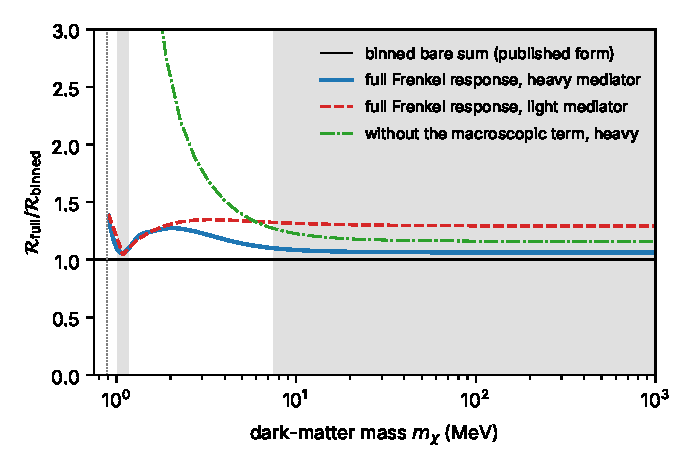
\includegraphics[width=0.85\linewidth]{figures/ch16/limit16_4a.pdf}
\captionof{figure}{Rate of the full Frenkel-exciton response of anthracene divided by the binned rate, against the dark-matter mass, for a heavy (solid) and a light (dashed) mediator, direction-averaged halo. Full response: all 49 $\pi$-electron singlets on both molecules, coupled by $\mathfrak{J}$ and by the macroscopic Coulomb term $(e^2/\Omega q^2)F F^\dagger$, so that no factor $1/|\varepsilon_{\mathrm{mac}}|^2$ is needed (\cref{app:D.12}); the molecular levels are shifted by \SI{0.27}{eV} so that the lowest optically allowed exciton at $\vect{Q} \to 0$ lies at the measured \SI{3.1}{eV} of the binned form. Dash-dotted: the full response without the macroscopic term, heavy mediator. Model of \cref{sec:16.4-model}, $\pi$ electrons only. Gray: the heavy-mediator ratio within \SI{10}{\percent} of one. Dotted: the binned threshold, \SI{0.883}{MeV}.}\label{fig:16-limit-frenkel}
\par}
\smallskip
Just above threshold, between 0.88 and \SI{1.0}{MeV}, the lowest exciton of the full model lies below the binned line and the ratio reaches 1.38. For a heavy mediator between 1.2 and \SI{7.5}{MeV}, and for a light mediator at every mass above \SI{1.2}{MeV}, the mixing of the weak $L_a$ line with the strong $B_b$ transition and the dispersion of the exciton bands change the rate by 10 to \SI{35}{\percent}; the incoherent sum contains neither effect.
\end{limitbox}

Above \SI{30}{MeV} the heavy-mediator rate of the full response in \cref{fig:16-limit-frenkel} exceeds the binned one by \SI{6.3}{\percent}, flat in mass; this excess is the intensity borrowing of \cref{eq:16.4-borrow}. Since $\mathfrak{J}$ is periodic in the crystal momentum, its $L_a$--$B_b$ element keeps the binned weight off by several percent at any momentum transfer. The element is \SI{0.12}{eV} at $\vect{Q} \to 0$ and \SI{0.18}{eV} at a general point of the zone, against an $L_a$--$B_b$ energy difference of \SI{1.4}{eV}. A light mediator weights the momentum transfers near the threshold value $\omega/v_{\mathrm{max}} = \SI{1.17}{keV}$, where $qa_{\mathrm{mol}} \approx 1.6$ for the root-mean-square radius $a_{\mathrm{mol}} = \SI{2.66}{\angstrom}$ of the carbon frame, and there the full rate exceeds the binned one by 29 to \SI{35}{\percent} at all masses above \SI{2}{MeV}. Between 1.2 and \SI{7.5}{MeV} the heavy-mediator ratio reaches 1.27, because the exciton bands spread the levels over tenths of an eV while the halo factor, near threshold, changes on that scale.

The dash-dotted curve shows that the macroscopic term matters most: without it, the local fields alone would raise the rate ninefold at \SI{1.1}{MeV}. The $\pi$ transitions themselves make $\varepsilon_{\mathrm{mac}}(q,0) - 1 = 0.83$ at the threshold momentum and 0.51 at \SI{2}{keV} in the model, so that the factor $1/|\varepsilon_{\mathrm{mac}}|^2$ of \cref{eq:16.4-S} cannot be applied line by line. In the full response the macroscopic term shifts weight up in energy instead of removing it (\cref{sec:4.9}).

\subsection{Charge-transfer excitons and other corrections}\label{sec:16.4-ct}

The zero-overlap limit removes the charge-transfer pairs, and real molecular crystals have some overlap. The simplest description keeps one Frenkel state $|\mathrm{Fr}\rangle$, of energy $E_{\mathrm{Fr}}$, and one charge-transfer state $|\mathrm{CT}\rangle$, of energy $E_{\mathrm{CT}}$, with the electron on a neighbor at distance $d$. The two are coupled by the transfer integral $t_{\mathrm{CT}}$, the sum of the integrals that move the electron and the hole between the molecules. The electron and hole transfer integrals are both proportional to the overlap of the orbitals of the two molecules. Diagonalizing the $2\times2$ problem gives two states $|\pm\rangle$ rotated by the mixing angle $\theta_{\mathrm{CT}}$,
\begin{equation}
  \tan2\theta_{\mathrm{CT}} = \frac{2t_{\mathrm{CT}}}{E_{\mathrm{CT}} - E_{\mathrm{Fr}}} , \qquad
  f_\pm(\vect{q}) = \cos\theta_{\mathrm{CT}}\,f_{\mathrm{Fr}}(\vect{q}) \pm \sin\theta_{\mathrm{CT}}\,f_{\mathrm{CT}}(\vect{q}) ,
  \label{eq:16.4-CT}
\end{equation}
with $f_{\mathrm{CT}}$ the form factor of the charge-transfer state. The transition density of the charge-transfer state is the overlap density of an empty orbital on one molecule and an occupied orbital on the other; it integrates to zero for orthogonal orbitals, so $f_{\mathrm{CT}}(0) = 0$; its dipole is of order $d$ times the overlap, and $|f_{\mathrm{CT}}|^2$ enters at order $q^2d^2$. In the rate the Frenkel line loses the fraction $\sin^2\theta_{\mathrm{CT}}$ of its weight to a new line near $E_{\mathrm{CT}}$, and a binned rate sees this shift of weight up in energy only if the bin ends between the two lines. And $f_{\mathrm{CT}}$ carries the phase difference between two molecules, and the charge-transfer contribution is coherent over distances of order $d$; no Frenkel model contains this coherence. In anthracene the charge-transfer pairs lie near the fundamental gap, 3.9--\SI{4.2}{eV}, some 0.8--\SI{1.1}{eV} above the lowest singlet~\cite[Tables~II and~III]{rangel2016structural}, and for small mixing $\theta_{\mathrm{CT}}^2 \simeq t_{\mathrm{CT}}^2/(E_{\mathrm{CT}} - E_{\mathrm{Fr}})^2$: a transfer integral of \SI{0.1}{eV} would move about one percent of the weight. The mixing grows along the acene series, whose larger members have singlets that extend over several molecules~\cite[Sect.~III\,E]{rangel2016structural}.

The nuclei move when a molecule is excited, and each molecular line becomes a Franck--Condon progression of vibronic replicas with Poisson weights set by a Huang--Rhys factor (\cref{eq:5.6-FC}). In the Condon approximation the progression keeps the total weight of the line, so \cref{eq:16.4-binned} holds for windows that cover it, while the Franck--Condon overlaps narrow the exciton band of each replica. Above the fundamental gap the crystal has a continuum of separated electrons and holes that the Frenkel model lacks, and \cref{eq:16.4-rate} omits it, as the published rates do~\cite{blanco2020dark}; this continuum raises the rate of masses above $2\times\SI{4}{eV}/v_{\mathrm{max}}^2 \approx \SI{1.1}{MeV}$. Triplet excitons cost less, \SI{1.9}{eV} for the lowest triplet of crystalline anthracene~\cite[Table~III]{rangel2016structural}, but a spin-independent density coupling cannot create them, and they enter only through the spin couplings of \cref{sec:10.4}. Finally, the $\pi$-electron model fails at momentum transfers above about \SI{10}{keV}, where the $\sigma$ electrons of the C--C and C--H bonds start to contribute to $|f|^2$. No calculation of the full periodic Bethe--Salpeter response of anthracene at finite $\vect{q}$ exists to compare with the binned molecular sum and with the zero-overlap model.

\subsection{Direction dependence of an anthracene target}\label{sec:16.4-aniso}

A $\pi$ orbital is odd under reflection through the molecular plane, so the transition density between two $\pi$ orbitals is even, and with zero differential overlap it is a sum of atomic densities centered in the plane. For $\vect{q}$ along the normal every phase $\ee^{\ii\vect{q}\cdot\vect{R}_\mu}$ is then the same, and $f = F_{2p}\sum_\mu \varrho_\mu$ vanishes. With the overlap densities kept and the measured, slightly puckered geometry, $|f|^2$ of $L_a$ at $q = \SI{2.07}{keV}$ is $1\times10^{-7}$ along the normal, against $0.25$ along the short axis. The transition density of $L_a$ also changes sign under reflection through the long axis, so that $|f|^2$ along that axis is only $2\times10^{-9}$. Near threshold, where only $L_a$ is reached, the molecule responds to the component of $\vect{q}$ along its short axis alone. In the crystal both short axes lie within \ang{27} of $b$, and the halo makes $\vect{q}$ prefer the direction of the wind when $\vmin$ is close to $v_{\mathrm{max}}$ (\cref{sec:11.7}): the rate is largest when the Earth moves along $b$.

\Cref{fig:16-anthracene} shows the rate of \cref{eq:16.4-rate} in the model, with the 20 singlets below \SI{7.5}{eV}, for the Earth's velocity along each crystal axis. At \SI{10}{MeV} and $\sigmae = \SI{e-37}{cm^2}$ the direction-averaged rate is $8.0\times10^4$ events per kg-year for a heavy mediator and $2.3\times10^4$ for a light one. The heavy-mediator value is comparable to the independent-particle rate of silicon, $1.36\times10^5$ (\cref{sec:10.2}). At \SI{1.0}{MeV}, just above threshold, $L_a$ carries the whole rate, and the largest rate over all directions of the wind, at $\hat{\vect{v}}_{\mathrm{E}} \parallel b$, exceeds the smallest, near the long molecular axes, 92 times for a heavy mediator and 69 times for a light one. The contrast falls quickly with the mass: $L_a$ carries \SI{68}{\percent} of the rate at \SI{2}{MeV} and \SI{19}{\percent} at \SI{10}{MeV}, as $B_b$ and the higher levels fill in the directions $L_a$ cannot use. The ratio of the largest to the smallest rate is 2.3 (heavy) and 5.3 (light) at \SI{1.5}{MeV}, 1.20 and 1.39 at \SI{10}{MeV}, and 1.17 and 1.29 above \SI{100}{MeV}.

\begin{figure}[tbp]
  \centering
  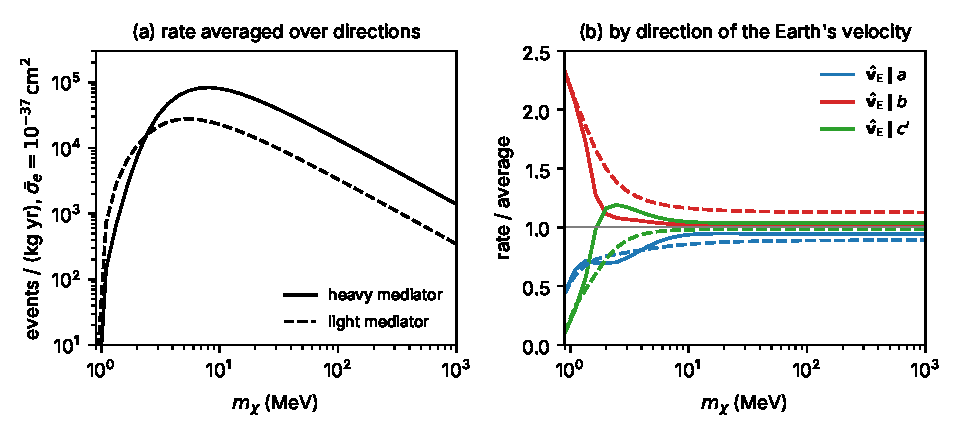
\includegraphics[width=\linewidth]{figures/ch16/fig16_4.pdf}
  \caption{Frenkel-exciton rate of an anthracene crystal in the binned form \cref{eq:16.4-rate}, per kg-year at $\sigmae = \SI{e-37}{cm^2}$, standard halo of \cref{tab:1-shm}. (a) Rate averaged over the directions of the Earth's velocity $\hat{\vect{v}}_{\mathrm{E}}$, heavy (solid) and light (dashed, $\FDM = (\alpha m_e/q)^2$) mediator. (b) Rate for $\hat{\vect{v}}_{\mathrm{E}}$ along the crystal axes $a$, $b$ and $c'$ (perpendicular to $a$ and $b$), divided by the average; heavy (solid) and light (dashed) mediator. The rate is even in $\hat{\vect{v}}_{\mathrm{E}}$. Model of \cref{sec:16.4-model}: $\pi$-electron singlets below \SI{7.5}{eV} of the Pariser--Parr--Pople model on the measured crystal structure, lowest singlet at \SI{3.1}{eV}, form factors with zero differential overlap; the continuum above the fundamental gap is not included.}
  \label{fig:16-anthracene}
\end{figure}

Whatever the mounting and the latitude, $\hat{\vect{v}}_{\mathrm{E}}$ sweeps only part of the sphere in a sidereal day, and the amplitude $A_{\mathrm{day}}$ of \cref{eq:11.7-Aday} cannot exceed $(\mathcal{R}_{\mathrm{max}} - \mathcal{R}_{\mathrm{min}})/(\mathcal{R}_{\mathrm{max}} + \mathcal{R}_{\mathrm{min}})$ over all directions. In the model this bound is 0.98 (heavy) and 0.97 (light) at \SI{1.0}{MeV}, 0.39 and 0.68 at \SI{1.5}{MeV}, 0.09 and 0.17 at \SI{10}{MeV}, and 0.08 and 0.13 at \SI{1}{GeV}. The bound near threshold is a hundred times the daily modulation of silicon, \SI{0.9}{\percent} at \SI{2}{MeV} (\cref{we:11-daily}), because of the crystal class. A cubic crystal has no quadrupole, and its first anisotropic term, the hexadecapole $\ell = 4$, passes the halo only at a few percent; in monoclinic anthracene the quadrupole $\ell = 2$ is allowed and passes at tens of percent of $\mathcal{H}_0$ (\cref{eq:11.7-ups}). Blanco et al.\ reach the same conclusion for trans-stilbene, with a modulation near one at threshold and, at large masses, a modulation above the ten percent of the annual modulation~\cite[Sects.~V, VI]{blanco2021dark}.
